% =====================================================================
%  RELATÓRIO PIBIT — MODELO EM LaTeX
%  Espelha o formato do relatório PIBIC/UnB (A4, ABNT, Arial 12, 1,5)
%  e a estrutura das "Instruções para escrita de trabalhos científicos".
%
%  Overleaf: Menu > Compilador = pdfLaTeX. Bibliografia = BibTeX (padrão).
%  Leia o arquivo LEIAME.md antes de começar.
% =====================================================================
\documentclass[12pt,a4paper]{article}

% =====================================================================
%  PREÂMBULO — formatação. Em geral não é preciso mexer aqui.
% =====================================================================

% ---------- Idioma e codificação ----------
\usepackage[T1]{fontenc}
\usepackage[utf8]{inputenc}
\IfFileExists{brazilian.ldf}{\usepackage[english,brazilian]{babel}}{\usepackage[english]{babel}}

% ---------- Fonte Arial (equivalente livre: Helvetica) ----------
\usepackage[scaled=0.92]{helvet}
\renewcommand{\familydefault}{\sfdefault}
\usepackage{microtype}

% ---------- Página: A4, margens 3 cm (sup./esq.) e 2 cm (inf./dir.) ----------
\usepackage[a4paper,top=3cm,left=3cm,bottom=2cm,right=2cm]{geometry}

% ---------- Espaçamento 1,5 e recuo de 1,25 cm ----------
\usepackage{setspace}
\onehalfspacing
\setlength{\parindent}{1.25cm}
\setlength{\parskip}{0pt}
\usepackage{indentfirst}

% ---------- Pacotes gerais ----------
\usepackage{amsmath,amssymb}
\usepackage{siunitx}
\sisetup{output-decimal-marker={,}, group-separator={.}, per-mode=symbol}
\usepackage{graphicx}
\graphicspath{{figuras/}}
\usepackage{booktabs,tabularx,array,multirow}
\usepackage{float}
\usepackage[dvipsnames]{xcolor}
\usepackage{tikz}
\usetikzlibrary{positioning,arrows.meta,shapes.geometric,fit}
\usepackage{enumitem}
\setlist{nosep,leftmargin=1.25cm}
\usepackage{ifthen}
\newboolean{rascunho}

% ---------- Títulos: "1 INTRODUÇÃO" (12 pt, negrito, maiúsculas) ----------
\usepackage{titlesec}
\titleformat{\section}{\normalsize\bfseries}{\thesection}{0.5em}{\MakeUppercase}
\titleformat{\subsection}{\normalsize\bfseries}{\thesubsection}{0.5em}{}
\titleformat{\subsubsection}{\normalsize\bfseries\itshape}{\thesubsubsection}{0.5em}{}
\titlespacing*{\section}{0pt}{12pt}{6pt}
\titlespacing*{\subsection}{0pt}{12pt}{6pt}
\titlespacing*{\subsubsection}{0pt}{6pt}{6pt}
% Seções sem número (RESUMO, ABSTRACT, REFERÊNCIAS...)
\newcommand{\secaosemnumero}[1]{%
  \section*{#1}\addcontentsline{toc}{section}{#1}}

% ---------- Legendas: "Figura 1 — Título" (10 pt, centralizada) ----------
\usepackage{caption}
\captionsetup{font=small,labelsep=endash,justification=centering,singlelinecheck=false,skip=6pt}
\captionsetup[table]{position=top}
\DeclareCaptionLabelSeparator{travessao}{\ --\ }
\captionsetup{labelsep=travessao}
% Fonte abaixo da figura/tabela: \fonte{Autor (2026).}
\newcommand{\fonte}[1]{\par\vspace{4pt}{\centering\small\linespread{1}\selectfont Fonte: #1\par}}

% Novos ambientes flutuantes usados nos modelos: Quadro e Gráfico
\usepackage{newfloat}
\DeclareFloatingEnvironment[fileext=loq,listname={Lista de Quadros},name=Quadro,placement=htbp]{quadro}
\DeclareFloatingEnvironment[fileext=log2,listname={Lista de Gráficos},name=Gráfico,placement=htbp]{grafico}
\captionsetup[quadro]{position=top}

% Nomes em português independentemente do idioma carregado
\AtBeginDocument{%
  \renewcommand{\figurename}{Figura}%
  \renewcommand{\tablename}{Tabela}%
  \renewcommand{\abstractname}{Resumo}%
}

% ---------- Siglas (Dica 4: por extenso na 1.ª vez, depois só a sigla) ----------
\usepackage[printonlyused,nohyperlinks]{acronym}

% ---------- Links (precisa vir ANTES do abntex2cite) ----------
\usepackage[hidelinks]{hyperref}

% ---------- Citações ABNT: \citeonline{chave} -> Autor (2025); \cite{chave} -> (AUTOR, 2025) ----------
\IfFileExists{abntex2cite.sty}{%
  \usepackage[alf,abnt-emphasize=bf,abnt-etal-cite=2,abnt-etal-list=0,abnt-and-type=e]{abntex2cite}%
  \citebrackets()%
}{%
  \usepackage[round,authoryear]{natbib}
  \newcommand{\citeonline}{\citet}
  \bibliographystyle{plainnat}
}

% ---------- Orientações de escrita (somem quando rascunho = false) ----------
\newcommand{\escrever}[1]{%
  \ifthenelse{\boolean{rascunho}}{{\color{BrickRed}\itshape [Escrever: #1]}}{}}
\newcommand{\dica}[1]{%
  \ifthenelse{\boolean{rascunho}}{%
    \par\noindent\fcolorbox{BrickRed}{red!4}{\parbox{\dimexpr\linewidth-2\fboxsep-2\fboxrule}{\small\color{BrickRed}\textbf{Orientação:} #1}}\par}{}}


% ---------------------------------------------------------------------
% RASCUNHO: true mostra as orientações em vermelho no PDF.
% Troque para false quando for entregar (todas as orientações somem).
% ---------------------------------------------------------------------
\setboolean{rascunho}{true}

% ---------------------------------------------------------------------
% DADOS DO TRABALHO
% ---------------------------------------------------------------------
\newcommand{\titulo}{MINIATURIZAÇÃO E INTEGRAÇÃO DE SENSORES TÁTEIS MAGNÉTICOS eFLESH EM UMA LUVA COM FEEDBACK VIBROTÁTIL}
\newcommand{\autor}{Artur Ferreira Gonçalves}
\newcommand{\orientador}{Prof. Dr. Felix}
\newcommand{\departamento}{Faculdade de Tecnologia (FT) -- UnB}
\newcommand{\laboratorio}{Laboratório de Visualização, Interação e Simulação -- L-VIS}
\newcommand{\programa}{PIBIT -- Programa Institucional de Bolsas de Iniciação em Desenvolvimento Tecnológico e Inovação -- 2026/2027}

\begin{document}

% ------------------------- CABEÇALHO --------------------------------
\begin{center}
  \begin{spacing}{1.5}
    {\fontsize{14}{18}\selectfont\bfseries \titulo\par}
  \end{spacing}
  \vspace{0.6cm}
  \autor\par
  \vspace{0.3cm}
  \orientador\par
  \departamento\par
  \laboratorio\par
  \programa\par
\end{center}
\vspace{0.5cm}

% ------------------------- ELEMENTOS PRÉ-TEXTUAIS --------------------
% =====================================================================
%  RESUMO E ABSTRACT — escreva POR ÚLTIMO (Item 4 das instruções).
%  Pergunta-guia: "O que eu fiz em poucas palavras?"
%  Conteúdo: objetivo (IDÊNTICO ao da Introdução — Dica 7), método e
%  resultados mais relevantes. Um parágrafo, espaçamento simples.
% =====================================================================
\secaosemnumero{RESUMO}
\begin{spacing}{1.0}
\noindent
\escrever{contexto em 1--2 frases: luvas medem movimento, mas não a força nas pontas dos dedos.}
\escrever{objetivo, copiado da Introdução: Este trabalho tem como objetivo ...}
\escrever{método em 2--3 frases: projeto da microestrutura cut-cell em TPU, magnetômetro TLV493D, caracterização em bancada, calibração por regressão e MLP, integração com feedback vibrotátil.}
\escrever{principais resultados com números: RMSE de força em N, faixa útil, latência.}
\escrever{contribuição em 1 frase.}

\vspace{6pt}
\noindent Palavras-chave: Sensor tátil magnético; eFlesh; Manufatura aditiva; Feedback vibrotátil; Aprendizado de máquina.
\end{spacing}

\secaosemnumero{ABSTRACT}
\begin{spacing}{1.0}
\noindent
\begin{otherlanguage}{english}
\escrever{tradução fiel do Resumo para o inglês.}
\end{otherlanguage}

\vspace{6pt}
\noindent Keywords: Magnetic tactile sensor; eFlesh; Additive manufacturing; Vibrotactile feedback; Machine learning.
\end{spacing}


% Lista de siglas (Dica 4). Só aparecem as siglas efetivamente usadas.
% =====================================================================
%  LISTA DE SIGLAS
%  Use no texto: \ac{ERM} -> 1.ª vez "Motor de Massa Excêntrica Rotativa (ERM)",
%  depois só "ERM". Plural: \acp{MLP}. Forçar a forma longa: \acl{MLP}.
%  Só aparecem na lista as siglas realmente usadas no texto.
% =====================================================================
\secaosemnumero{LISTA DE SIGLAS}
\begin{spacing}{1.0}
\begin{acronym}[TCA9548A]
  \acro{CAD}{Desenho Assistido por Computador}
  \acro{CEP}{Comitê de Ética em Pesquisa}
  \acro{ERM}{Motor de Massa Excêntrica Rotativa}
  \acro{ESP32}{microcontrolador ESP32 da Espressif}
  \acro{FDM}{Modelagem por Fusão e Deposição}
  \acro{I2C}{Inter-Integrated Circuit}
  \acro{L-VIS}{Laboratório de Visualização, Interação e Simulação}
  \acro{LRA}{Atuador Ressonante Linear}
  \acro{MLP}{Perceptron Multicamadas}
  \acro{PCB}{Placa de Circuito Impresso}
  \acro{PWM}{Modulação por Largura de Pulso}
  \acro{RMSE}{Raiz do Erro Quadrático Médio}
  \acro{RV}{Realidade Virtual}
  \acro{TEMAC}{Teoria do Enfoque Meta-Analítico Consolidado}
  \acro{TPU}{Poliuretano Termoplástico}
\end{acronym}
\end{spacing}


% ------------------------- ELEMENTOS TEXTUAIS ------------------------
% =====================================================================
%  1 INTRODUÇÃO — "Qual é o problema da pesquisa?"
%  Ordem: contextualização -> problema -> questão de pesquisa (em forma de
%  pergunta) -> objetivo geral e específicos -> justificativa (pode virar
%  seção própria, como no modelo do INCRA) -> estrutura do trabalho.
%  Escrita SEMPRE impessoal (Dica 1): "propõe-se", "foi realizado".
% =====================================================================
\section{Introdução}

\escrever{contextualização: luvas sensorizadas capturam o movimento das mãos, mas raramente medem forças de contato nas pontas dos dedos; sensores resistivos de baixo custo sofrem com histerese, deriva e baixa repetibilidade. Citar a literatura, p.\,ex. \citeonline{dahiya2010tactile} e \citeonline{vanwegen2023haptics}.}

\escrever{estado da técnica em 1 parágrafo: sensores táteis magnéticos e o eFlesh \cite{pattabiraman2025eflesh}, com os números de desempenho reportados.}

\escrever{problema: o eFlesh foi demonstrado em blocos de 40$\times$40~mm, com cinco magnetômetros; não há relato da versão em escala de ponta de dedo humano nem da integração de múltiplas unidades em uma luva.}

\escrever{questão de pesquisa em forma de pergunta. Exemplo de estrutura: É possível miniaturizar ... mantendo ...?}

\escrever{objetivo geral (o MESMO texto que irá para o Resumo — Dica 7).}

Como objetivos específicos, propõem-se:
\begin{enumerate}[label=\alph*)]
  \item \escrever{projetar e fabricar por manufatura aditiva a microestrutura em escala de ponta de dedo;}
  \item \escrever{caracterizar em bancada a resposta a força normal, cisalhante e posição de contato;}
  \item \escrever{calibrar e comparar modelos de regressão e \ac{MLP} com validação temporal;}
  \item \escrever{embarcar o modelo no microcontrolador e fechar a malha com feedback vibrotátil;}
  \item \escrever{validar o conjunto em tarefas com objetos reais.}
\end{enumerate}

\escrever{justificativa: relevância técnica e social (caso de uso que justifica o feedback no mundo real).}

\escrever{estrutura do trabalho: Este trabalho está organizado da seguinte forma: a Seção~\ref{sec:estado-arte} apresenta ...; a Seção~\ref{sec:referencial} ...; a Seção~\ref{sec:metodo} ...; a Seção~\ref{sec:resultados} ...; e a Seção~\ref{sec:conclusoes} ...}

% =====================================================================
%  2 LEVANTAMENTO DO ESTADO DA ARTE — "O que já foi falado sobre isso?"
%  Instruções (Item 1 e Dica 9): revisão sistemática pelo TEMAC
%  (www.pesquisatemac.com), em bases indexadas, com:
%   - palavras-chave e bases usadas;
%   - análises de co-citação (co-citation) e acoplamento (coupling);
%   - quadro-resumo com as pesquisas e autores principais;
%   - modelo integrador e análise crítica (mostrar o GAP).
%  Referências atualizadas: preferir os últimos 4 anos.
%  Alternativa aceita: protocolo PRISMA (como no artigo de RA veicular).
%  Se faltar espaço (formato de artigo), substitua por "Trabalhos
%  relacionados" ao fim do Referencial Teórico.
% =====================================================================
\section{Levantamento do Estado da Arte}\label{sec:estado-arte}

\escrever{parágrafo de ligação com a Introdução (Dica 2).}

\subsection{Protocolo da revisão}

\escrever{bases consultadas (Web of Science, Scopus, IEEE Xplore), período, string de busca, número de registros em cada etapa do TEMAC.}

\dica{A string pode partir das buscas já feitas, por exemplo: ("magnetic tactile sensor" OR "Hall effect tactile") AND ("3D print*" OR "microstructure" OR "glove"). Registre o número de resultados de cada base.}

\subsection{Análises de co-citação e acoplamento}

\escrever{resultados do TEMAC: principais periódicos, autores, países e as frentes de pesquisa identificadas pelo acoplamento bibliográfico. Inserir as figuras geradas (VOSviewer) com Figura e Fonte.}

\subsection{Quadro-resumo}

O Quadro~\ref{qua:estado-arte} reúne as pesquisas de maior aderência ao tema.
\escrever{completar e revisar o quadro com os trabalhos selecionados.}

\begin{quadro}[H]
  \caption{Principais pesquisas sobre sensores táteis magnéticos}
  \label{qua:estado-arte}
  \begin{spacing}{1.0}\footnotesize
  \begin{tabularx}{\linewidth}{|>{\raggedright\arraybackslash}p{2.9cm}|>{\raggedright\arraybackslash}X|>{\raggedright\arraybackslash}X|}
    \hline
    \textbf{Referência} & \textbf{Abordagem} & \textbf{Principal resultado} \\ \hline
    \citeonline{bhirangi2021reskin} & Pele elastomérica com partículas magnéticas sobre 5 magnetômetros & Pele substituível; auto-supervisão reduz a perda de desempenho entre peças \\ \hline
    \citeonline{bhirangi2024anyskin} & Pele autoaderente e alinhada & Menor variação entre unidades e troca da pele em segundos \\ \hline
    \citeonline{kristanto2018wearable} & Sensores Hall nas laterais da ponta do dedo humano & Força 3D sem cobrir a polpa; compensação do campo terrestre \\ \hline
    \citeonline{pattabiraman2025eflesh} & Microestrutura cut-cell impressa em TPU com ímãs embutidos & RMSE de 0,27~N (normal) e 0,12~N (cisalhante) \\ \hline
    \citeonline{barthel2026eflesh} & Regressão polinomial aplicada ao eFlesh & RMSE de 0,09~N sem rede neural \\ \hline
    \escrever{...} & & \\ \hline
  \end{tabularx}
  \fonte{Elaborado pelo autor (2026).}
  \end{spacing}
\end{quadro}

\subsection{Modelo integrador e análise crítica}

\escrever{figura que integra os achados (por exemplo: transdução $\times$ fabricação $\times$ calibração $\times$ aplicação) e análise crítica mostrando a lacuna: ausência de versão em escala de dedo humano, uso de um único magnetômetro, interferência do atuador vibrotátil não caracterizada e falta de protocolos padronizados de avaliação.}

% =====================================================================
%  3 REFERENCIAL TEÓRICO — "Quais conceitos subsidiam o trabalho?"
%  Cada subseção deve terminar ligando-se à seguinte (Dica 2), e todas
%  devem ter relação direta com os resultados.
%  Tabelas/figuras sempre citadas pelo número: "conforme a Tabela 1".
% =====================================================================
\section{Referencial Teórico}\label{sec:referencial}

\escrever{parágrafo de abertura explicando a sequência dos conceitos.}

\subsection{Sensoriamento tátil}
\escrever{tecnologias de transdução (resistiva, capacitiva, piezoelétrica, óptica e magnética) e por que a magnética é adequada à ponta do dedo \cite{dahiya2010tactile}.}

\subsection{Efeito Hall e magnetômetros tridimensionais}
\escrever{princípio do efeito Hall; campo de um ímã permanente e decaimento com a distância; características do TLV493D \cite{infineon2016tlv493d}: faixa, resolução, endereçamento \ac{I2C}.}

\begin{equation}
  B_z(z) = \frac{B_r}{2}\left[\frac{z+L}{\sqrt{R^2+(z+L)^2}} - \frac{z}{\sqrt{R^2+z^2}}\right]
  \label{eq:campo-disco}
\end{equation}
\escrever{explicar cada símbolo da Equação~\eqref{eq:campo-disco} (campo axial de um ímã em disco).}

\subsection{Microestruturas e manufatura aditiva em TPU}
\escrever{microestruturas cut-cell \cite{tozoni2024cutcell}, rigidez controlada pela geometria \cite{panetta2015elastic}, comportamento do \ac{TPU} impresso sob compressão \cite{bates2016honeycombs}.}

\subsection{Calibração por aprendizado de máquina}
\escrever{regressão linear e polinomial; \ac{MLP}; métricas (\ac{RMSE}, R$^2$); validação temporal e vazamento de dados \cite{bergmeir2012crossvalidation}; inferência embarcada \cite{david2021tflm}.}

\subsection{Feedback vibrotátil}
\escrever{mecanorreceptores e percepção de vibração; atuadores \ac{ERM} e \ac{LRA} \cite{culbertson2018haptics}; acionamento por \ac{PWM}.}

% =====================================================================
%  4 MÉTODO DE PESQUISA — "Como resolvi o problema?"
%  Dois tópicos (Item 3): (1) classificação da pesquisa;
%  (2) estruturação, SEMPRE representada por uma Figura (Dica 5).
%  As etapas daqui viram as subseções dos Resultados (Dica 6).
% =====================================================================
\section{Método de Pesquisa}\label{sec:metodo}

\escrever{parágrafo de ligação com o Referencial Teórico.}

\subsection{Classificação da pesquisa}

\escrever{natureza (aplicada), abordagem (quantitativa), objetivos (exploratória e experimental) e procedimentos (pesquisa experimental em laboratório). Descrever amostras: número de sensores fabricados, número de ensaios, número de voluntários (se houver), instrumentos de medição e técnicas de análise.}

\dica{Se houver testes com voluntários, citar a aprovação do \ac{CEP} (Resolução CNS 466/2012) e colocar o termo de consentimento no Apêndice.}

\subsection{Estruturação da pesquisa}

A pesquisa foi estruturada em sete etapas, conforme a Figura~\ref{fig:estrutura}.
\escrever{ajustar o texto e a figura às etapas reais.}

\begin{figure}[H]
  \centering
  \begin{spacing}{1.0}
  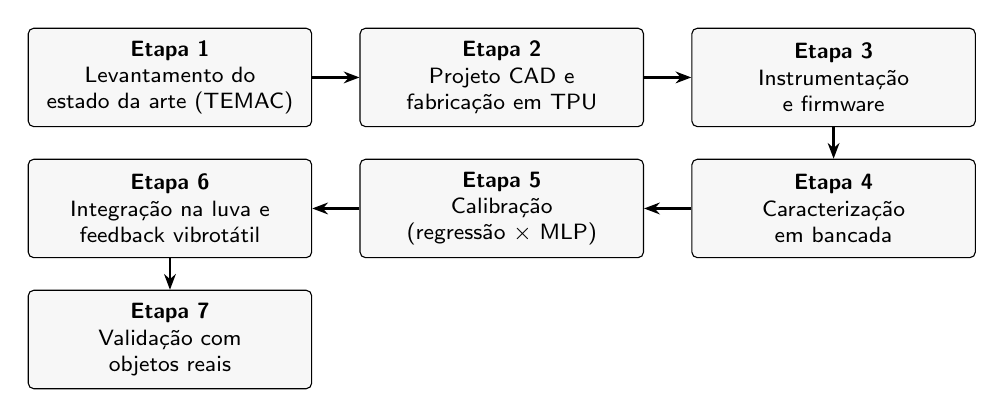
\begin{tikzpicture}[
      node distance=4mm and 6mm,
      etapa/.style={draw, rounded corners=2pt, align=center, font=\footnotesize,
                    minimum width=3.6cm, minimum height=1.25cm, fill=gray!6},
      seta/.style={-{Stealth[length=2mm]}, thick}]
    \node[etapa] (e1) {\textbf{Etapa 1}\\Levantamento do\\estado da arte (TEMAC)};
    \node[etapa, right=of e1] (e2) {\textbf{Etapa 2}\\Projeto CAD e\\fabricação em TPU};
    \node[etapa, right=of e2] (e3) {\textbf{Etapa 3}\\Instrumentação\\e firmware};
    \node[etapa, below=of e3] (e4) {\textbf{Etapa 4}\\Caracterização\\em bancada};
    \node[etapa, left=of e4] (e5) {\textbf{Etapa 5}\\Calibração\\(regressão $\times$ MLP)};
    \node[etapa, left=of e5] (e6) {\textbf{Etapa 6}\\Integração na luva e\\feedback vibrotátil};
    \node[etapa, below=of e6] (e7) {\textbf{Etapa 7}\\Validação com\\objetos reais};
    \draw[seta] (e1) -- (e2);
    \draw[seta] (e2) -- (e3);
    \draw[seta] (e3) -- (e4);
    \draw[seta] (e4) -- (e5);
    \draw[seta] (e5) -- (e6);
    \draw[seta] (e6) -- (e7);
  \end{tikzpicture}
  \end{spacing}
  \caption{Estruturação da pesquisa}
  \label{fig:estrutura}
  \fonte{Elaborado pelo autor (2026).}
\end{figure}

\subsubsection{Etapa 1 -- Levantamento do estado da arte}
\escrever{como a revisão TEMAC foi conduzida (detalhes na Seção~\ref{sec:estado-arte}).}

\subsubsection{Etapa 2 -- Projeto CAD e fabricação}
\escrever{dimensões (15$\times$15$\times$10~mm), tamanho de célula, espessura das paredes, critério de imprimibilidade (bico de 0,4~mm), filamento \ac{TPU} 95A, ímãs N52, pausa de impressão para inserção dos ímãs.}

\subsubsection{Etapa 3 -- Instrumentação e firmware}
\escrever{TLV493D na lateral da falange distal, multiplexador TCA9548A, \ac{ESP32}, taxa de amostragem, linha de base ($\Delta B$), arquitetura modular do firmware.}

\subsubsection{Etapa 4 -- Caracterização em bancada}
\escrever{instrumento de referência (célula de carga), faixas de força normal (0--15~N) e cisalhante (0--8~N), malha de localização 10$\times$10~mm, número de repetições, controle de temperatura.}

\subsubsection{Etapa 5 -- Calibração}
\escrever{modelos comparados, divisão dos dados por ensaio (validação temporal), métricas, exportação do modelo para o microcontrolador.}

\subsubsection{Etapa 6 -- Integração e feedback vibrotátil}
\escrever{posição dos motores \ac{ERM} (dorso ou palma), driver MOSFET, mapeamento força $\rightarrow$ \ac{PWM}, teste de interferência magnética em função da distância, medição de latência.}

\subsubsection{Etapa 7 -- Validação}
\escrever{tarefas (aperto controlado, detecção de deslizamento e pinça fina), condição de comparação, métricas e critério de sucesso.}

% =====================================================================
%  5 RESULTADOS E DISCUSSÃO — "O que descobri? O que isso significa?"
%  É a essência do trabalho e o principal critério de avaliação.
%  As subseções seguem EXATAMENTE as etapas do Método (Dica 6).
%  Para cada etapa: o que foi obtido (tabular os dados) + análise crítica.
%  Resultados negativos e soluções de contorno também são resultados
%  (veja como o relatório do INCRA trata a limitação do Autodesk Tandem).
% =====================================================================
\section{Resultados e Discussão}\label{sec:resultados}

\escrever{parágrafo de abertura: o que esta seção apresenta e como está organizada.}

\subsection{Estado da arte}
\escrever{síntese dos achados da Etapa 1 que orientaram as decisões de projeto.}

\subsection{Fabricação dos sensores}
\escrever{fotos dos protótipos (Figura), parâmetros finais, falhas de impressão e ajustes.}

\subsection{Instrumentação e firmware}
\escrever{leitura do sensor, ruído medido, estabilidade da linha de base.}

\subsection{Caracterização em bancada}
\escrever{curvas força $\times$ $\Delta B$ (Gráfico), histerese, repetibilidade.}

\subsection{Calibração}

A Tabela~\ref{tab:modelos} compara os modelos de calibração.
\escrever{substituir pelos resultados com o sensor fabricado.}

\begin{table}[H]
  \centering
  \caption{Erro de estimativa de força por modelo de calibração}
  \label{tab:modelos}
  \begin{spacing}{1.0}\small
  \begin{tabular}{lccc}
    \toprule
    \textbf{Modelo} & \textbf{RMSE (N)} & \textbf{R$^2$} & \textbf{Parâmetros} \\
    \midrule
    Regressão linear              & -- & -- & 4 \\
    Regressão polinomial (grau 2) & -- & -- & 10 \\
    MLP 2$\times$16               & -- & -- & 353 \\
    MLP 2$\times$128              & -- & -- & 17.153 \\
    \bottomrule
  \end{tabular}
  \fonte{Elaborado pelo autor (2026).}
  \end{spacing}
\end{table}

\escrever{discussão: qual modelo foi escolhido para o ESP32 e por quê, comparando com \citeonline{pattabiraman2025eflesh} e \citeonline{barthel2026eflesh}.}

\subsection{Integração e feedback vibrotátil}
\escrever{interferência do ERM em função da distância (Gráfico), latência da malha, consumo.}

\subsection{Validação}
\escrever{desempenho nas tarefas com objetos reais.}

\subsection{Discussão}
\escrever{o que os resultados significam diante da literatura; limitações encontradas e por quê.}

% =====================================================================
%  6 CONSIDERAÇÕES FINAIS — "O objetivo foi atendido?"
%  Resgatar a questão de pesquisa e o objetivo da Introdução e mostrar
%  que foram respondidos; resumir os principais resultados; qualificar
%  as hipóteses (verdadeiras, falsas, inconsistentes ou indeterminadas);
%  apresentar limitações e sugestões de trabalhos futuros.
% =====================================================================
\section{Considerações Finais}\label{sec:conclusoes}

\escrever{retomar a questão de pesquisa e responder diretamente.}

\escrever{mostrar, objetivo específico por objetivo específico, que foram atingidos, com os números principais.}

\escrever{contribuição do trabalho.}

\escrever{limitações da pesquisa.}

\escrever{trabalhos futuros: por exemplo, PCB própria, integração com ambientes de \ac{RV} (Unity/ROS2) via Wi-Fi/BLE, testes com mais usuários.}


% ------------------------- ELEMENTOS PÓS-TEXTUAIS --------------------
% =====================================================================
%  AGRADECIMENTOS — "Quem me ajudou?" Citar o órgão de fomento.
% =====================================================================
\secaosemnumero{AGRADECIMENTOS}

\escrever{agradecer ao órgão de fomento da bolsa PIBIT (CNPq ou UnB/DPI, conforme o edital), ao \ac{L-VIS} e ao orientador.}


\secaosemnumero{REFERÊNCIAS}
\begin{spacing}{1.0}
  \bibliography{referencias}
\end{spacing}

% =====================================================================
%  APÊNDICES E ANEXOS
%  Apêndice = material de fonte primária, produzido pelo autor
%  (termo de consentimento, roteiro de testes, código, desenhos).
%  Anexo = material de terceiros (datasheets, dados abertos).
%  Apague esta seção se não houver nada a anexar.
% =====================================================================
\clearpage
\appendix
\renewcommand{\thesection}{APÊNDICE \Alph{section}}
\titleformat{\section}{\normalsize\bfseries}{\thesection\ --}{0.5em}{\MakeUppercase}

\section{Lista de materiais}
\escrever{tabela resumida da BOM ou referência ao repositório.}

\section{Roteiro dos testes com objetos reais}
\escrever{protocolo das tarefas de aperto, deslizamento e pinça.}


\end{document}
